% TensoraX final IEEE report (two-column). Build: docs/report/build_report.sh
% Numbers come from numbers.tex (scripts/make_report_numbers.py); figures from figures/ (scripts/make_report_figures.py).
\documentclass[conference]{IEEEtran}
\usepackage{mathptmx}
\usepackage{amsmath}
\usepackage{graphicx}
\usepackage{booktabs}
\usepackage{array}
\usepackage{cite}
\usepackage{xspace}
\usepackage[hidelinks]{hyperref}
% Generated by scripts/make_report_numbers.py - do not edit by hand.
\newcommand{\CpuName}{Apple M3\xspace}
\newcommand{\CompilerName}{Apple clang version 21.0.0\xspace}
\newcommand{\BenchDate}{2026-11-22\xspace}
\newcommand{\Trials}{9\xspace}
\newcommand{\TimerNs}{41\xspace}
\newcommand{\GhzLo}{3.8\xspace}
\newcommand{\GhzHi}{4.0\xspace}
\newcommand{\MatmulsPerTrialM}{4.8\xspace}
\newcommand{\VecOutputs}{5{,}400\xspace}
\newcommand{\VecRecords}{600\xspace}
\newcommand{\VecMismatches}{0\xspace}
\newcommand{\HeadCyc}{51\xspace}
\newcommand{\HeadCycLo}{51\xspace}
\newcommand{\HeadCycHi}{52\xspace}
\newcommand{\HeadNs}{12.9\xspace}
\newcommand{\HeadS}{7.3\xspace}
\newcommand{\HeadMacCyc}{0.53\xspace}
\newcommand{\BestCyc}{18\xspace}
\newcommand{\BestNs}{4.7\xspace}
\newcommand{\BestS}{2.6\xspace}
\newcommand{\BestMacCyc}{1.46\xspace}
\newcommand{\OzeroCyc}{223\xspace}
\newcommand{\OzeroS}{31.8\xspace}
\newcommand{\OzeroNs}{56\xspace}
\newcommand{\HeadLatCyc}{57\xspace}
\newcommand{\HeadLatS}{8.2\xspace}
\newcommand{\BestLatCyc}{33\xspace}
\newcommand{\BestLatS}{4.7\xspace}
\newcommand{\SLo}{2.6\xspace}
\newcommand{\SHi}{37.8\xspace}
\newcommand{\HwMacCyc}{3.86\xspace}
\newcommand{\FmaxLo}{92.97\xspace}
\newcommand{\FmaxHi}{93.68\xspace}
\newcommand{\FmaxLoShort}{93.0\xspace}
\newcommand{\FTarget}{200\xspace}
\newcommand{\HwNsMeasured}{75.3\xspace}
\newcommand{\HwNsTarget}{35.0\xspace}
\newcommand{\CpuFasterHead}{5.8\xspace}
\newcommand{\CpuFasterBest}{15.9\xspace}
\newcommand{\CpuFasterOzero}{1.3\xspace}
\newcommand{\CpuFasterHeadTarget}{2.7\xspace}
\newcommand{\CpuFasterBestTarget}{7.4\xspace}
\newcommand{\GflopsCpuHead}{4.2\xspace}
\newcommand{\GflopsCpuBest}{11.4\xspace}
\newcommand{\GflopsHwMeasured}{0.72\xspace}
\newcommand{\GflopsHwTarget}{1.54\xspace}
\newcommand{\ClockRatio}{43\xspace}
\newcommand{\CrossN}{11\xspace}
\newcommand{\CrossNTarget}{8\xspace}
\newcommand{\SixteenCyc}{3923\xspace}
\newcommand{\SixteenS}{85.3\xspace}
\newcommand{\SixteenHw}{46\xspace}
\newcommand{\SweepThreeCyc}{53\xspace}
\newcommand{\SweepThreeS}{7.5\xspace}
\newcommand{\EtaThree}{42.9\xspace}
\newcommand{\EtaLimit}{33.3\xspace}
\newcommand{\EtaBatchHundred}{98.7\xspace}
\newcommand{\EtaBatchTen}{88.2\xspace}
\newcommand{\TrafficRatioThree}{2.33\xspace}
\newcommand{\TrafficRatioSixteen}{11.00\xspace}
\newcommand{\TrafficRatioThreeBit}{2.0\xspace}
\newcommand{\TrafficRatioSixteenBit}{8.5\xspace}
\newcommand{\XDsp}{9\xspace}
\newcommand{\XLut}{576\xspace}
\newcommand{\XCarry}{72\xspace}
\newcommand{\XFF}{482\xspace}
\newcommand{\XIbuf}{100\xspace}
\newcommand{\XObuf}{288\xspace}
\newcommand{\XBufg}{1\xspace}
\newcommand{\XLutTwo}{288\xspace}
\newcommand{\XLutFour}{9\xspace}
\newcommand{\XLutFive}{279\xspace}
\newcommand{\EMult}{9\xspace}
\newcommand{\ECarry}{144\xspace}
\newcommand{\ELut}{292\xspace}
\newcommand{\EFF}{482\xspace}
\newcommand{\FmaxSeedOne}{93.32\xspace}
\newcommand{\FmaxSeedTwo}{92.97\xspace}
\newcommand{\FmaxSeedThree}{93.68\xspace}
\newcommand{\TableCpuRows}{-O0 generic & 223 & 31.8 & 264 & 37.8 \\
-O0 fixed-3 & 222 & 31.7 & 265 & 37.8 \\
-O2 generic \textbf{(headline)} & 51 & 7.3 & 57 & 8.2 \\
-O2 fixed-3 & 18 & 2.6 & 33 & 4.7 \\
-O3 generic & 40 & 5.7 & 43 & 6.2 \\
-O3 fixed-3 & 19 & 2.7 & 33 & 4.7 \\}
\newcommand{\TableTrafficRows}{2 & 40 & 24 & 1.67 & 1.50 & 0.67 \\
3 & 126 & 54 & 2.33 & 2.00 & 1.00 \\
4 & 288 & 96 & 3.00 & 2.50 & 1.33 \\
8 & 2{,}176 & 384 & 5.67 & 4.50 & 2.67 \\
16 & 16{,}896 & 1{,}536 & 11.00 & 8.50 & 5.33 \\}


\newcommand{\tx}{TensoraX\xspace}
\hyphenation{Tensora-X accu-mu-la-tor}

\begin{document}

\title{TensoraX: A 3$\times$3 Output-Stationary Systolic Array for Matrix Multiplication --- RTL Design, FPGA Synthesis and CPU Benchmarking}

\author{\IEEEauthorblockN{Adnan Rizvi, Aviral Mishra, Praanshu Ranjan, and Aditya Pal}
\IEEEauthorblockA{\textit{Modern Computer Architecture Project, Rishihood University, India}}}

\maketitle

\begin{abstract}
\tx is a Verilog 3$\times$3 output-stationary systolic array that multiplies signed 16-bit matrices with nine multiply-accumulate processing elements and 32-bit accumulators. This paper adds synthesis, benchmarking and scaling results to our earlier RTL and simulation study. A 3$\times$3 product completes in 7 clock cycles ($3N-2$); an RTL timing test confirms $3N-2$ for $N=2$ to $8$. Yosys maps the core to \XDsp DSP48E1 slices, \XLut LUTs and \XFF flip-flops on the Artix-7 family. Place-and-route on a Lattice ECP5 proxy closes at \FmaxLo--\FmaxHi~MHz, below the \FTarget~MHz target, so Artix-7 timing remains unmeasured. A sequential C baseline, verified bit-exact against the RTL test vectors, needs about \HeadCyc cycles per 3$\times$3 product on one \CpuName core, i.e.\ $S=\HeadS\times$ more cycles than \tx; its best optimised form needs about \BestCyc cycles ($S=\BestS\times$). In wall-clock time, however, the CPU is \CpuFasterHead{}$\times$ faster than the \FmaxLoShort~MHz prototype, because it runs at about \ClockRatio{}$\times$ the clock. Because the clear signal is broadcast to all PEs, tiles must start $3N-2$ cycles apart, so sustained PE utilisation is \EtaThree{}\% and not the \EtaBatchHundred{}\% of a pipelined bound. We state the assumptions behind every comparison.
\end{abstract}

\begin{IEEEkeywords}
Systolic array, matrix multiplication, FPGA synthesis, benchmarking, roofline model, output-stationary dataflow.
\end{IEEEkeywords}

\section{Introduction}
Matrix multiplication dominates the arithmetic of many machine-learning workloads. A conventional processor repeatedly moves operands between memory and registers, and this data movement, the memory wall, can cost more time and energy than the arithmetic itself. Systolic arrays attack the problem by forwarding each operand between neighbouring processing elements (PEs) in a clocked rhythm, so an operand fetched once is used many times \cite{kung1982,kungleiserson}.

\tx is a compact, parameterised Verilog array. Our Phase~1 study established its functional correctness in RTL simulation but reported no synthesis, timing or performance comparison. This paper closes that gap. Its contributions are:
\begin{enumerate}
\item Synthesis results on the Artix-7 family (Yosys) and routed timing on a Lattice ECP5 proxy (nextpnr), with the limits of that proxy stated (Section~\ref{sec:synth}).
\item A sequential CPU baseline with the same arithmetic as the RTL, checked bit-exact against the RTL regression vectors, and a speedup $S=\text{CPU cycles}/7$ reported together with the wall-clock comparison it does not capture (Section~\ref{sec:cpu}).
\item RTL timing checks showing a latency of $3N-2$ cycles for $N=2\ldots8$ and a minimum tile spacing of $3N-2$ cycles for the current clear scheme, which fixes the sustained utilisation of the design as built (Section~\ref{sec:util}).
\item A consolidated scaling, external-traffic and roofline discussion with the assumptions behind each model (Section~\ref{sec:traffic}).
\end{enumerate}
The main finding is deliberately two-sided. In clock cycles \tx is \HeadS{}$\times$ better than a straightforward C loop; in time, an \CpuName core at about 4~GHz beats our \FmaxLoShort~MHz FPGA prototype on a single 3$\times$3 product. The architectural benefit shows up in cycle count, traffic and scaling, not in raw time at $N=3$.

\section{Related Work}
Kung and Leiserson introduced systolic arrays as regular networks of simple cells that pass data rhythmically \cite{kungleiserson}, and Kung later argued for their regularity, modularity and balance of computation and communication \cite{kung1982}. Jouppi et al.\ describe the Google TPU, whose matrix-multiply unit is a weight-stationary systolic array \cite{tpu}; \tx is output-stationary, which keeps partial sums in place at the cost of streaming both operands. Williams et al.\ proposed the Roofline model, which bounds attainable performance by the lesser of peak arithmetic rate and memory bandwidth times operational intensity \cite{roofline}; we use it in Section~\ref{sec:traffic}. The TPU's reported performance does not transfer to a 3$\times$3 educational prototype, and we make no such claim.

\section{Design, Verification and Method}
\subsection{Architecture}
The top module \texttt{systolic\_array\_3x3} instantiates $N\times N$ PEs ($N=3$). Each PE holds a signed 16$\times$16 multiplier, a 32-bit accumulator, and registers that forward the activation east and the weight south. Row $i$ of $A$ is injected $i$ cycles late and column $j$ of $B$ is injected $j$ cycles late, so $A_{i,k}$ and $B_{k,j}$ meet at PE$(i,j)$. The last accumulation, at PE$(N-1,N-1)$, completes $3N-2$ cycles after the first feed edge. A single synchronous clear, \texttt{clr\_acc}, and the asynchronous reset are broadcast to all PEs. Table~\ref{tab:params} lists the parameters.

\begin{table}[!t]
\caption{TensoraX parameters}
\label{tab:params}
\centering\footnotesize
\begin{tabular}{@{}ll@{}}
\toprule
Array & 3$\times$3, nine PEs, orthogonal mesh \\
Operands / accumulator & signed 16-bit / signed 32-bit (wraps) \\
Dataflow & output-stationary, skewed feed \\
Clear & \texttt{clr\_acc} broadcast to all PEs \\
Latency of one tile & 7 cycles ($3N-2$) \\
Ports & \texttt{a\_rows} 48 b, \texttt{b\_cols} 48 b, \texttt{c\_flat} 288 b \\
\bottomrule
\end{tabular}
\end{table}

\subsection{Verification environment}
All array testbenches run in Icarus Verilog. The regression has seven items: a PE unit test, a directed array test, a 600-operation randomised test whose expected values come from an independent Python model, a 13-test corner-case suite, an overflow demonstration, the Python PE reference model, and the analytical scaling models. A cycle-level assertion checker watches every PE on every clock edge, and a mutation script injects seven bugs into a copy of the RTL to confirm the tests catch them \cite{repo}.

\subsection{FPGA flow}
Resource counts come from Yosys 0.71 (\texttt{synth\_xilinx -family xc7 -flatten}), synthesis only \cite{yosys}. Timing comes from \texttt{synth\_ecp5} followed by nextpnr-ecp5 0.11.1 \cite{nextpnr} on a LFE5U-85F, speed grade 6, out-of-context, a single clock with a 200~MHz target, three placer seeds, register-to-register paths only. The synthesised RTL is byte-identical to the RTL in the repository at the time of writing (SHA-256 in \texttt{docs/synthesis/MANIFEST.txt}).

\subsection{CPU baseline method}
\label{sec:method}
The baseline (\texttt{scripts/cpu\_baseline.c}) computes $C=AB$ with a triple loop, 16-bit signed operands and a 32-bit wrapping accumulator, the same function as the RTL. Both loop variants (\emph{generic}: $N$ read at run time; \emph{fixed-3}: $N=3$ known to the compiler) reproduce all \VecOutputs outputs of the \VecRecords RTL regression vectors with \VecMismatches mismatches at every optimisation level. Each configuration is timed over about \MatmulsPerTrialM million products per trial, \Trials trials, and the median is reported. Two workloads are used: \emph{throughput}, independent products from an L1-resident pool that the out-of-order core can overlap; and \emph{latency}, where each result feeds the next product and every product waits for the previous one. Timer granularity is \TimerNs~ns, small against a trial of tens of milliseconds.

No user-space cycle counter is available on the test machine, so cycles are an \emph{estimate}: ns per product times a clock estimate (\GhzLo--\GhzHi~GHz across configurations) obtained from a chain of one-cycle dependent adds run before and after every trial. We defined the headline configuration before measuring: generic loop, \texttt{-O2}, throughput workload. The speedup is
\begin{equation}
S=\frac{\text{CPU cycles per 3$\times$3 product}}{7},
\end{equation}
and we also report the wall-clock ratio $t_\text{CPU}/t_\text{HW}$ with $t_\text{HW}=7/f_\text{HW}$. The conditions are: (i) the 7 cycles are one tile from first feed edge to final accumulation with operands already at the array boundary, so no memory or host transfer is included; (ii) the CPU runs one thread of scalar code from L1-resident data (the compiler emitted no SIMD instructions for these kernels, as disassembly shows); (iii) the CPU cycle count is estimated as above; (iv) for \tx one tile per 7 cycles is both its latency and its throughput, because tiles cannot overlap (Section~\ref{sec:util}).

\section{Results and Discussion}
\subsection{Functional verification}
Table~\ref{tab:verif} summarises the verification state of the repository head, re-run for this paper.

\begin{table}[!t]
\caption{Verification results (Icarus Verilog)}
\label{tab:verif}
\centering\footnotesize
\begin{tabular}{@{}p{0.50\columnwidth}p{0.42\columnwidth}@{}}
\toprule
Item & Result \\
\midrule
Regression (7 items) & all pass \\
Randomised array test & 600 operations, 5,400 outputs, 0 errors \\
Corner-case suite & 13 of 13 pass \\
Assertion checker & 422,316 checks, 0 failures \\
Bug injection & 7 of 7 mutants killed$^{\dagger}$ \\
CPU kernels vs.\ RTL vectors & 5,400 outputs, 0 mismatches \\
\bottomrule
\end{tabular}

\vspace{2pt}\raggedright\scriptsize $^{\dagger}$The mutation script uses GNU \texttt{sed}; on macOS we ran it with a GNU-compatible \texttt{sed} on the path (all seven mutations applied and were caught).
\end{table}

\subsection{FPGA synthesis and timing}
\label{sec:synth}
Table~\ref{tab:synth} gives the Artix-7-family resource counts and the routed timing.

\begin{table}[!t]
\caption{Synthesis and timing (core only)}
\label{tab:synth}
\centering\footnotesize
\begin{tabular}{@{}p{0.40\columnwidth}p{0.52\columnwidth}@{}}
\toprule
\multicolumn{2}{@{}l}{\emph{Artix-7 family, Yosys (synthesis only)}} \\
DSP48E1 & \XDsp (one per PE) \\
LUTs & \XLut (LUT2 \XLutTwo, LUT4 \XLutFour, LUT5 \XLutFive) \\
CARRY4 / flip-flops & \XCarry / \XFF \\
I/O buffers & \XIbuf in, \XObuf out (core, no board) \\
\midrule
\multicolumn{2}{@{}l}{\emph{Lattice ECP5 proxy, nextpnr, routed}} \\
Mapping & \EMult MULT18X18D, \ECarry CCU2C, \ELut LUT4, \EFF FFs \\
Fmax, seeds 1/2/3 (MHz) & \FmaxSeedOne / \FmaxSeedTwo / \FmaxSeedThree \\
At 200~MHz target & fails on all three seeds \\
Artix-7 WNS and Fmax & \textbf{not measured} \\
\bottomrule
\end{tabular}
\end{table}

Each PE maps to one DSP48E1, as the architecture intends. The flip-flop count is below the 585 an untrimmed design would hold because synthesis removes unconnected east- and south-edge forwarding registers. The ECP5 critical path (seed~1) runs from a register at the multiplier input through the multiplier (3.93~ns of logic), 2.05~ns of routing, and the carry chain into the 32-bit accumulator: the product is formed and added in the same cycle. This is a different FPGA family, so it is a proxy and not an Artix-7 number. A pre-synthesis estimate of 263~MHz for Artix-7 appears in the design notes; it is an architectural estimate that this measurement neither confirms nor refutes, and we do not use it. Registering the multiplier output before the accumulate is the obvious fix, but it changes the RTL and the 7-cycle latency and was not tried.

\subsection{CPU versus \tx}
\label{sec:cpu}
Table~\ref{tab:cpu} gives cycles per 3$\times$3 product for six builds under both workloads. The headline configuration needs \HeadCyc cycles (spread \HeadCycLo--\HeadCycHi across trials), so $S=\HeadS$. The best optimised loop, with $N=3$ visible to the compiler, needs about \BestCyc cycles ($S=\BestS$); the unoptimised \texttt{-O0} loop needs \OzeroCyc cycles ($S=\OzeroS$). Over all twelve configurations $S$ ranges from \SLo to \SHi. In MACs per cycle, \tx sustains $27/7=\HwMacCyc$ as built, against \HeadMacCyc for the headline CPU loop and \BestMacCyc for the best one.

\begin{table}[!t]
\caption{Cycles per 3$\times$3 product, Apple M3 (median of \Trials trials) and $S$=cycles/7}
\label{tab:cpu}
\centering\footnotesize
\begin{tabular}{@{}lrrrr@{}}
\toprule
& \multicolumn{2}{c}{Throughput} & \multicolumn{2}{c}{Latency} \\
\cmidrule(lr){2-3}\cmidrule(lr){4-5}
Build \& loop & cycles & $S$ & cycles & $S$ \\
\midrule
\TableCpuRows
\bottomrule
\end{tabular}
\end{table}

These $S$ values are cycle ratios, not time ratios. The CPU clock is about \ClockRatio{}$\times$ the routed FPGA clock, so one product takes \HeadNs~ns on the CPU (headline) and \BestNs~ns at best, against $7/\FmaxLoShort~\text{MHz}=\HwNsMeasured$~ns for \tx: the CPU is \CpuFasterHead{}$\times$ faster (\CpuFasterBest{}$\times$ for the best loop, and still \CpuFasterOzero{}$\times$ for the unoptimised \texttt{-O0} loop). Even at the unmet 200~MHz target ($\HwNsTarget$~ns) the CPU would be \CpuFasterHeadTarget{}$\times$ faster (\CpuFasterBestTarget{}$\times$ for the best loop). Expressed as throughput, the CPU delivers \GflopsCpuHead--\GflopsCpuBest~GFLOP/s on this kernel against \GflopsHwMeasured~GFLOP/s for the prototype as built (\GflopsHwTarget~GFLOP/s at 200~MHz). A single 3$\times$3 tile is simply too small for nine PEs at tens of MHz to beat a wide out-of-order core at 4~GHz.

\begin{figure}[!t]
\centering
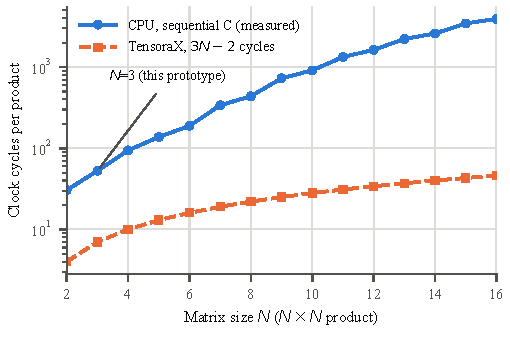
\includegraphics[width=\columnwidth]{figures/fig_cycles.pdf}
\caption{Cycles per $N\times N$ product. CPU: measured, generic \texttt{-O2} loop. \tx: $3N-2$, simulated in RTL for $N=2\ldots8$ and analytic beyond.}
\label{fig:cycles}
\end{figure}

Fig.~\ref{fig:cycles} extends the cycle comparison to $N=16$. The CPU needs \SweepThreeCyc cycles at $N=3$ in this independent sweep run (\HeadCyc in Table~\ref{tab:cpu}; the two runs of the same configuration differ by under 3\%) and \SixteenCyc at $N=16$, against $3N-2=\SixteenHw$ for \tx, so $S$ grows to \SixteenS. Fig.~\ref{fig:time} converts this to time. The hardware curves for $N\neq3$ are projections at the $N=3$ clock: a larger array would need $N^2$ DSP slices and would probably clock lower, so they are optimistic. On that basis the projected break-even is $N=\CrossN$ at the routed \FmaxLoShort~MHz and $N=\CrossNTarget$ at 200~MHz. The xc7a35t named in the project plan offers 90 DSP48E1 slices \cite{ds180}, so $N\le9$ fits by DSP count alone; at the routed clock the projection says the CPU stays ahead for every size that fits.

\begin{figure}[!t]
\centering
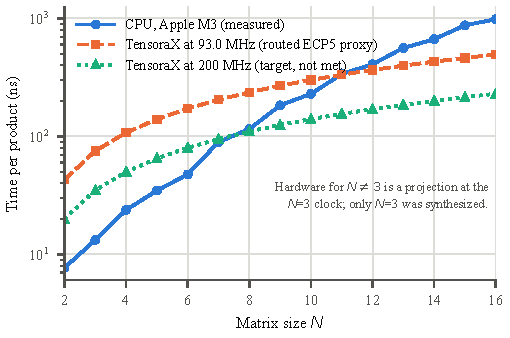
\includegraphics[width=\columnwidth]{figures/fig_walltime.pdf}
\caption{Time per product. CPU measured; \tx at the routed ECP5 clock and at the 200~MHz target (not met). Only $N=3$ was synthesised.}
\label{fig:time}
\end{figure}

\subsection{Latency, tile spacing and utilisation}
\label{sec:util}
A timing testbench feeds two tiles $S$ cycles apart with the normal skew and a broadcast clear at each tile start. A tile completes exactly $3N-2$ edges after its first feed edge for $N=2,\ldots,8$, and the corner PE is not yet complete one edge earlier. For $N=3$, spacings $S=3,4,5,6$ corrupt $8,6,3,1$ of the nine second-tile outputs, while $S\ge7$ is correct. The broadcast clear wipes accumulators that are still in mid-tile, or the next tile accumulates on top of the previous one. Tiles therefore cannot start closer than $3N-2$ cycles in the current RTL, and sustained utilisation is $N^3/(N^2(3N-2))=N/(3N-2)$, i.e.\ \EtaThree{}\% at $N=3$ falling toward \EtaLimit{}\% for large $N$ (Fig.~\ref{fig:util}).

\begin{figure}[!t]
\centering
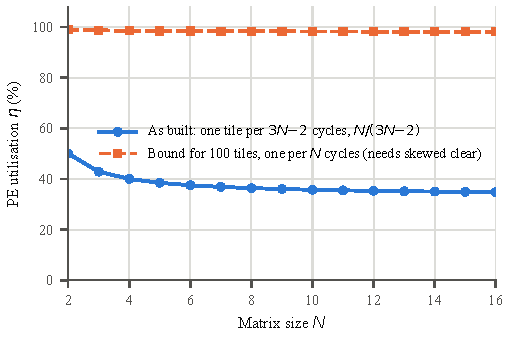
\includegraphics[width=\columnwidth]{figures/fig_util.pdf}
\caption{PE utilisation. The as-built curve follows from the tile-spacing test; the upper curve is the analytic bound for 100 tiles issued every $N$ cycles, which the current RTL does not support.}
\label{fig:util}
\end{figure}

The analytical batch-streaming model reaches \EtaBatchHundred{}\% for 100 tiles (\EtaBatchTen{}\% for 10) but assumes a new tile every $N$ cycles. Reaching it needs the clear to travel along the wavefront like the valid bit, plus staggered result capture. We have not implemented or simulated that, so we report \EtaThree{}\% as the measured property of the design and the higher figure only as a bound.

\subsection{External traffic and roofline}
\label{sec:traffic}
The traffic model (Adnan Rizvi's analysis in the repository) counts every operand load of a naive CPU loop as external traffic, $(2N^3+N^2)$ elements, against $3N^2$ elements for \tx, which reads each element of $A$ and $B$ once and writes $C$ once. With 2-byte elements the reduction is $(2N+1)/3$ (Table~\ref{tab:traffic}), i.e.\ \TrafficRatioThree{}$\times$ at $N=3$ and \TrafficRatioSixteen{}$\times$ at $N=16$. Two assumptions limit these numbers. First, the RTL writes back 32-bit accumulators; with 4-byte $C$ elements the ratio is $(N+1)/2$, i.e.\ \TrafficRatioThreeBit{}$\times$ at $N=3$ and \TrafficRatioSixteenBit{}$\times$ at $N=16$. Second, a real CPU caches: at $N=3$ all operands sit in registers or L1 and the compulsory traffic equals that of \tx, so the ratio applies to a cache-less machine, not to our measured baseline.

\begin{table}[!t]
\caption{Modelled external traffic (bytes, 2-byte elements) and operational intensity $I$ (FLOP/byte)}
\label{tab:traffic}
\centering\footnotesize
\begin{tabular}{@{}rrrrrr@{}}
\toprule
$N$ & CPU & \tx & ratio & ratio (32-bit $C$) & $I$ \\
\midrule
\TableTrafficRows
\bottomrule
\end{tabular}
\end{table}

\begin{figure}[!t]
\centering
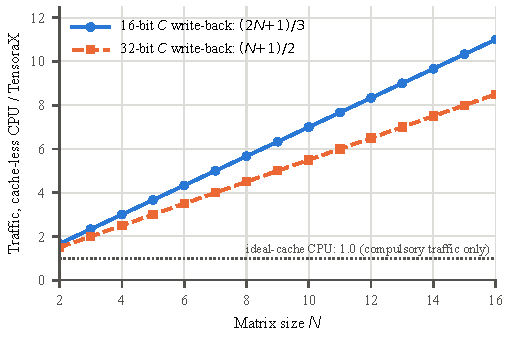
\includegraphics[width=\columnwidth]{figures/fig_traffic.pdf}
\caption{Modelled traffic reduction against a cache-less CPU, for 16-bit and 32-bit write-back of $C$.}
\label{fig:traffic}
\end{figure}

The roofline model gives an operational intensity $I=N/3$ FLOP/byte and, with a 200~MHz clock and 12.8~GB/s of bandwidth, a compute-bound regime up to $N=8$ and a memory-bound one at $N=16$ (68.3 of 102.4~GFLOP/s). Its peak assumes all $N^2$ PEs busy every cycle at 200~MHz, whereas the design as built sustains $N/(3N-2)$ of that and met only \FmaxLoShort~MHz after routing. The model therefore describes where the architecture could go, not what the prototype achieves.

\section{Limitations}
\begin{itemize}
\item \textbf{Timing.} Artix-7 WNS and Fmax were not measured; the ECP5 result is a proxy, single-clock, out-of-context and without I/O constraints. Resource counts are from synthesis only, and no place-and-route utilisation exists.
\item \textbf{Size.} Only $N=3$ was synthesised. Results for $N\neq3$ are analytic (latency simulated for $N\le8$).
\item \textbf{CPU baseline.} One machine, one compiler, one thread; cycles are estimated from a clock estimate. Hand-vectorised or library implementations were not measured and would be faster. The CPU figure is a steady-state loop; the \tx figure is one tile without data transfer.
\item \textbf{Traffic model.} Cache-less CPU and, in the original model, 16-bit write-back of $C$.
\item \textbf{Arithmetic.} The 32-bit accumulator wraps for extreme inputs (for example, three products of $(-32768)^2$); 33 bits suffice for $N=3$.
\item \textbf{No power or energy measurement.}
\end{itemize}

\section{Conclusion and Future Scope}
\tx computes a 3$\times$3 signed 16-bit matrix product in 7 cycles ($3N-2$, simulated for $N=2$ to $8$) on nine DSP-mapped PEs. It is functionally verified against an independent reference, and a sequential C implementation of the same function matches it bit for bit. Yosys maps it to \XDsp DSP48E1, \XLut LUTs and \XFF flip-flops on the Artix-7 family, and routed timing on an ECP5 proxy is \FmaxLo--\FmaxHi~MHz, short of the 200~MHz target. Against a straightforward C loop the array needs \HeadS{}$\times$ fewer cycles (\BestS{}$\times$ against the best loop), but a 4~GHz CPU core is still \CpuFasterHead{}$\times$ faster in time at $N=3$. As built, the broadcast clear limits utilisation to \EtaThree{}\%. The architecture's value at this stage lies in deterministic latency, nearest-neighbour wiring, reduced external traffic and cycle-count scaling, not in absolute speed.

Future work, in the order we would do it:
\begin{enumerate}
\item Implement on Artix-7 with the vendor tools to obtain real WNS, Fmax and utilisation, and constrain the I/O.
\item Register the multiplier output to shorten the critical path, and measure the effect on Fmax against the one-cycle latency cost.
\item Skew the clear and the result capture along the wavefront so a tile can start every $N$ cycles, then verify the pipelined utilisation bound in simulation.
\item Add a memory interface with double-buffered tiles to measure end-to-end performance, including data transfer.
\item Compare against vectorised CPU libraries and a GPU, and measure power.
\item Widen the accumulator or add saturation, and tile larger matrices onto the array (up to $N=9$ fits the xc7a35t by DSP count).
\end{enumerate}

\section*{Author Contributions}
Adnan Rizvi: microarchitecture, scaling and roofline analysis. Aviral Mishra: synthesis and timing. Praanshu Ranjan: array interconnect, CPU baseline, timing checks, report. Aditya Pal: visualisation and presentation. The verification suite (assertions, corner cases, mutation script) was written by Anurag Pandey in Phase~1. All numbers and Figs.~\ref{fig:cycles}--\ref{fig:traffic} in this paper are generated from committed tool outputs by \texttt{docs/report/build\_report.sh}.

\begin{thebibliography}{10}
\bibitem{kungleiserson} H. T. Kung and C. E. Leiserson, ``Systolic arrays for (VLSI),'' Carnegie-Mellon Univ., Dept.\ Comput.\ Sci., Tech.\ Rep.\ CMU-CS-79-103, Apr.\ 1978 (rev.\ Dec.\ 1978).
\bibitem{kung1982} H. T. Kung, ``Why systolic architectures?,'' \emph{Computer}, vol.~15, no.~1, pp.~37--46, Jan.\ 1982, doi: 10.1109/MC.1982.1653825.
\bibitem{tpu} N. P. Jouppi \emph{et al.}, ``In-datacenter performance analysis of a tensor processing unit,'' in \emph{Proc.\ 44th Annu.\ Int.\ Symp.\ Comput.\ Archit.\ (ISCA)}, 2017, pp.~1--12, doi: 10.1145/3079856.3080246.
\bibitem{roofline} S. Williams, A. Waterman, and D. Patterson, ``Roofline: An insightful visual performance model for multicore architectures,'' \emph{Commun.\ ACM}, vol.~52, no.~4, pp.~65--76, Apr.\ 2009, doi: 10.1145/1498765.1498785.
\bibitem{repo} Team TensoraX, ``TensoraX: 2D systolic array matrix multiplication accelerator,'' source code, scripts and documentation, GitHub, \url{https://github.com/adnan275/TensoraX}.
\bibitem{yosys} C. Wolf, ``Yosys open synthesis suite,'' \url{https://yosyshq.net/yosys/}.
\bibitem{nextpnr} YosysHQ, ``nextpnr portable FPGA place and route tool,'' \url{https://github.com/YosysHQ/nextpnr}.
\bibitem{ds180} Xilinx, ``7 series FPGAs data sheet: Overview,'' DS180.
\end{thebibliography}

\end{document}
